%1644
\newpage

\section{ジャンプアクションゲームに挑戦しよう}


\subsection{ジャンプアクションゲームのあそびかた}



ジャンプアップゲームでキャラクターを動かして遊ぶ\ruby{本格的}{ほん|かく|てき}なゲームを\ruby{体験}{たい|けん}してみましょう。


ファイル→「開く」メニューから「jump.hsp」を読み込んでください。

見つからない場合は、まわりの友達か、近くの先生に聞いてみてください。

[F5]キーで実行すると、タイトル画面が出ます。[Enter]キーを押して始めてください。


\begin{figure}[H]
    \begin{center}
      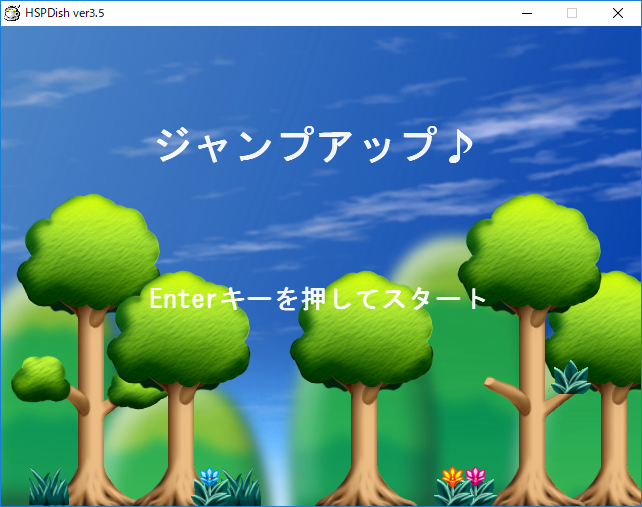
\includegraphics[keepaspectratio,width=11.192cm,height=8.827cm]{text04-img/s_jumptitle.png}
      \caption{タイトル画面}
    \end{center}
    \label{fig:prog_menu}
\end{figure}

ジャンプアップゲームは、キャラクターを操作してコインを取るゲームです。

左右の移動とジャンプをさせることができます。



\begin{figure}[H]
    \begin{center}
      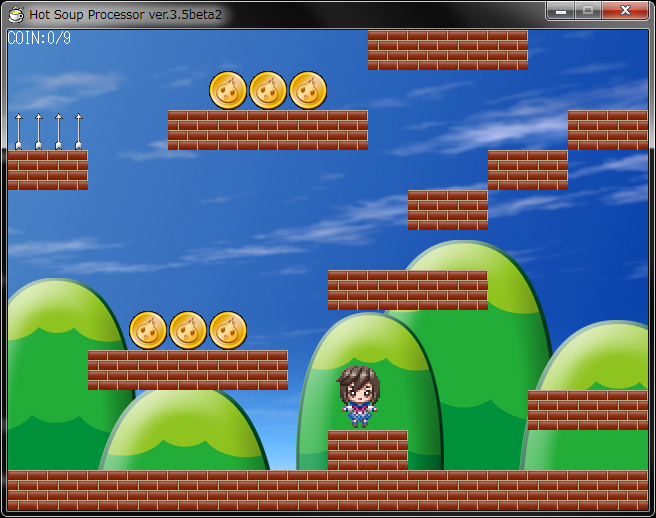
\includegraphics[keepaspectratio,width=11.28cm,height=8.915cm]{text04-img/s_jumpgame.png}
      \caption{ジャンプアップゲーム画面}
    \end{center}
    \label{fig:prog_menu}
\end{figure}

\ruby{矢印}{や|じるし}のキーで左右に動かして、スペースキーでジャンプです。

ジャンプしながら、コインを取って上に進みましょう。

すべてのコインを取るとあなたの勝ちです。逆に、\ruby{地面}{じ|めん}に置かれている\ruby{矢}{や}に当たってしまうとゲームオーバーになってしまいます。


\begin{figure}[H]
    \begin{center}
      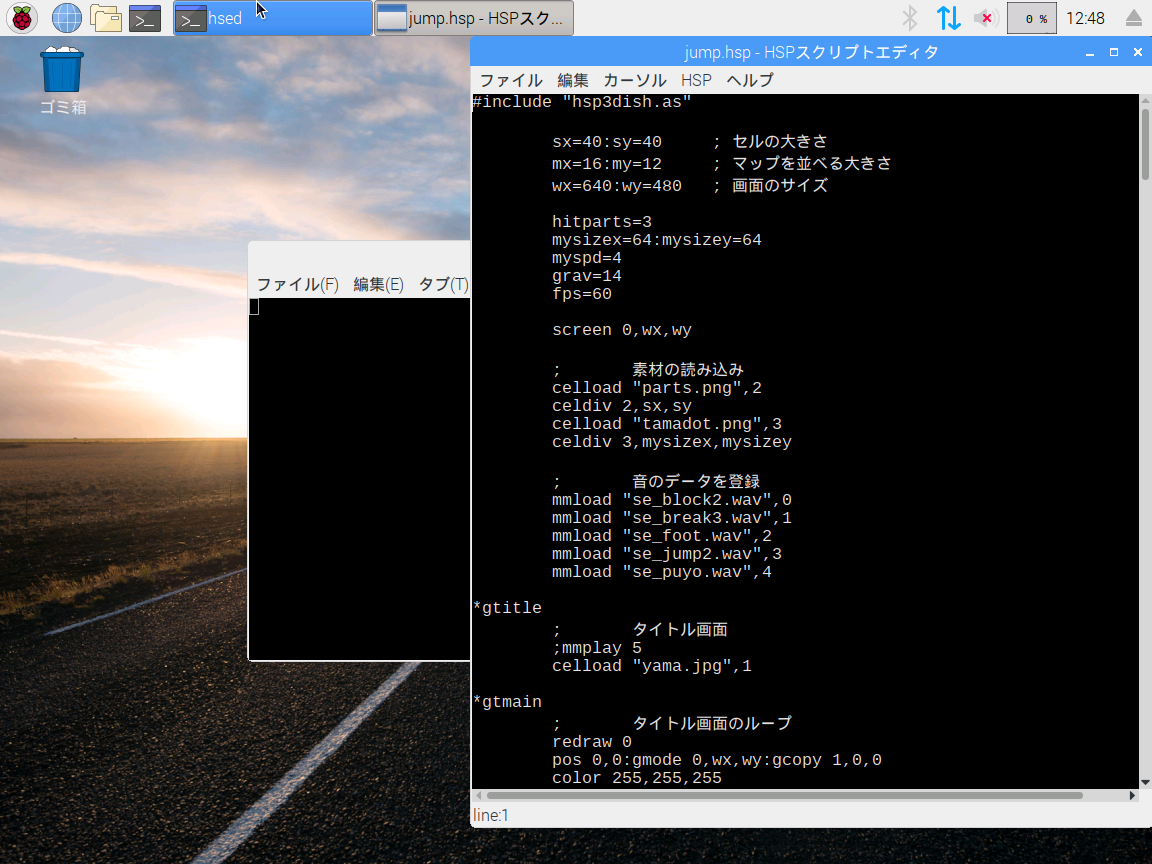
\includegraphics[keepaspectratio,width=11.192cm,height=8.393cm]{text04-img/text04-img024.png}
      \caption{ジャンプアップゲームのプログラム}
    \end{center}
    \label{fig:prog_menu}
\end{figure}

\newpage
\subsection{例題に挑戦しよう}

ゲームが遊べた人は、以下の例題にも挑戦してみよう。

・オリジナルの面を作ってみよう

・ゲームの動きを改造してみよう

・ゲームの背景や絵を改造してみよう

・ゲームのタイトル画面を改造してみよう

例題の考え方がわからない時は、近くのTAか先生に聞いてください。

わからない所は、そのままにせず、必ず答えを見つけてから先に進みましょう。

%1747